\documentclass[11pt,a4paper]{scrartcl}
\usepackage[margin=2.5cm]{geometry}
\usepackage[onehalfspacing]{setspace}
\usepackage{graphicx}
\usepackage[breaklinks=true,colorlinks=true,linkcolor=blue,urlcolor=blue,citecolor=blue]{hyperref}
\usepackage{amsmath,amsthm,amssymb}
\usepackage{icomma}
\usepackage[english]{babel}
\usepackage[T1]{fontenc}
\usepackage[space-before-unit=true,per-mode = symbol]{siunitx}
\usepackage{booktabs,multirow}
\usepackage{placeins}
\usepackage[natbib,abbreviate=true,doi=false,style=numeric-comp,giveninits=true,sorting=none]{biblatex}
\usepackage{csquotes} 
\addbibresource{MyBibliography.bib} 

\graphicspath{{Bilder/}}

\DeclareSIUnit{\dBm}{dBm}
\DeclareSIUnit[per-mode=reciprocal]\WN{\per\centi\meter}

\setlength{\parindent}{0pt}

\begin{document}
%
\title{Particle Detection in microscopy videos based on CNN}
\author{Jialin He, Yuanzhe Zhang, Dennis Kwong}
\date{\today}
\maketitle
\renewcommand\abstractname{Abstract}
\section*{\abstractname}
This is the final report for our MATH 509 group project. When given a microscopic video, true particles appear white while empty spaces appear black. Through thresholding in OpenCV, it is possible to roughly locate the locations of the particles. However, such approach does not suffice due to varying particle size, the existence of ``false'' particles, and does not give insights on particle movement tracking. Our group have thus used a machine learning approach - CNN to deal with the task, in addition to some other code snippets that could deal with the above issues.

\thispagestyle{empty}
\tableofcontents
\thispagestyle{empty}
\cleardoublepage
\pagenumbering{arabic} 
\newpage


%% SECTION 1 %%
\section{Introduction}
With better technology, microscope has higher magnifications and thus are able to record the movement of microscopic-sized particles. However, even with highly advanced microscopes, the issue of poor signal-to-noise ratios (i.e. high noise) could not be alleviated. Moreover, how to post-process microscopic videos and output the positions of particles on screen remains a hot topic in the machine learning and applied science community.\\

Our project is divided into two parts. First, before analyzing any microscopic videos, we have to find ways to turn mp4 videos into an array of data. This is done by OpenCV. In addition, after extracting the videos, we have attempted to perform basic analysis on the videos (i.e. part of Project Salmonella).\\

Second, we have generated training data via a python class. Since there are only limited number of microscope recordings, it is not realistic to train the neural network with those recordings. The python class generates video that roughly resembles a microscopic recording, with parameters including noise level, standard deviation of Brownian motion and particle size. The training data is then fed to train the CNN, which will later be used for particle detection (i.e. part of Project NeuralNet).


%% SECTION 2 %%
\section{Data processing}

In Project NeuralNet, no data was provided. In Project Salmonella, two types of data - tracks and videos were given. `Videos' data are mp4 videos captured by a microscope. The videos are 10 seconds long. `Tracks' data are csv files containing the $(x,y)$ coordinates of each particle in the videos at frame $t \in \{0,1,\dots, 159\}$.

\begin{table}[htbp]
\centering
\begin{tabular}{ccccc}
\toprule
\multicolumn{1}{c}{particle} & \multicolumn{1}{c}{$x$} & \multicolumn{1}{c}{$y$}	& \multicolumn{1}{c}{frame $t$} \\
\midrule
0 & 427.158 & 69.356 & 0 \\
0 & 427.128 & 69.407 & 1 \\
0 & 427.823 & 69.605 & 2 \\
$\vdots$ & $\vdots$ & $\vdots$ & $\vdots$ \\
\bottomrule
\end{tabular}
\caption{Data structure of `Tracks' dataset}
\end{table}


%% SECTION 2.1 %%
\subsection{OpenCV: A thresholding approach \& limitations}
Code for this part can be found in \url{Project NeuralNet/opencv_experiment.ipynb}.\\

Microscopy videos are stored in mp4 format, in which its pixel data could be translated and stored in an array by the help of OpenCV. By the \textit{cvtColor} method, a colorized video is turned interpreted as a grayscale video, and then converted into a matrix of values ranging from 0 to 255, representing each pixel's light intensity (0 being black, 255 being white). \\

OpenCV also provides a \textit{threshold} method. It stores all pixels with white intensity higher than the threshold to be 1, and others to be 0. 

$$\text{output pixel value} = \begin{cases}
    1 & \text{if pixel intensity} \geq \text{threshold}\\  
    0 & \text{if pixel intensity} < \text{threshold}
\end{cases}$$

Intuitively, in the video, particles appear white while empty space appears black. So upon setting a proper threshold, it is theoretically possible to detect which part of the image corresponds to particles, while which part is not. Upon testing this idea on a microscopic video, a major issue could be spotted.

\begin{figure}[h]
    \begin{center}
        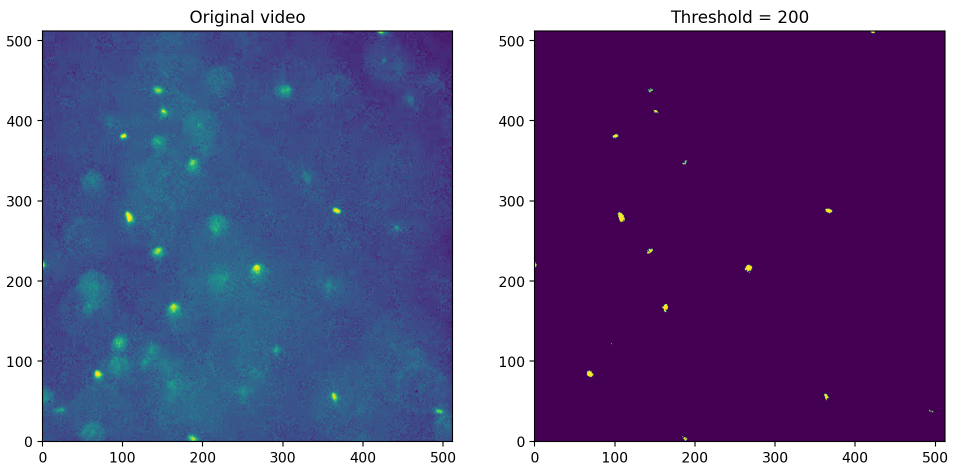
\includegraphics[width = 0.8\textwidth]{img/data200_t0.png}
    \end{center}
    \caption{Frame $t = 0$, Threshold $= 200$}
\end{figure}

The above shows the problem of over-filtering. Setting the threshold too high eliminates potential white spots, which could represent particles.

\begin{figure}[h]
    \begin{center}
        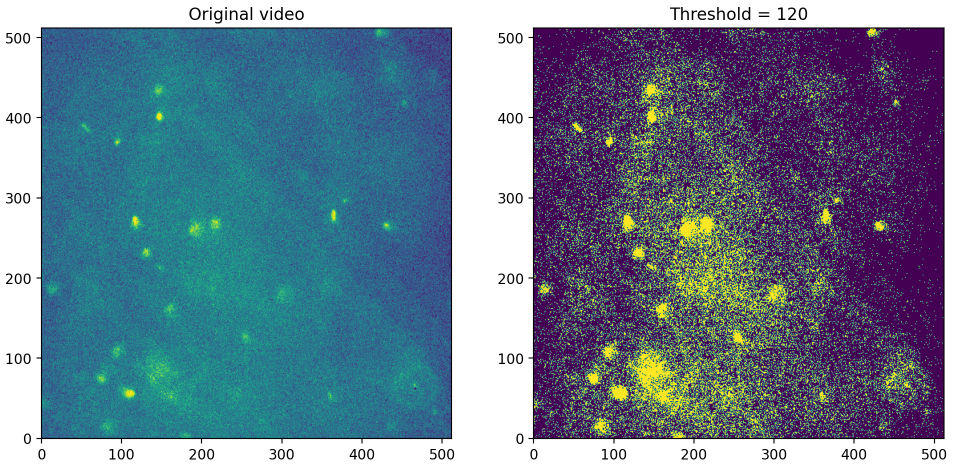
\includegraphics[width = 0.8\textwidth]{img/data120_t135.png}
    \end{center}
    \caption{Frame $t = 135$, Threshold $= 120$}
\end{figure}
 
On the other hand, setting the threshold too low would cause the map to be ``contaminated'' by noise. In frames with very high noise, the noise exceeds the threshold value, and thus gets a value of 1 in the map. This experiment gives us insights on why more advanced tools, such as neural networks, should be used instead.


%% SECTION 2.2 %%
\subsection{Interpretation of videos}
Code for this part can be found in \url{Project Salmonella/Project Salmonella.ipynb}, Goal 1.\\

We were provided with 27 recorded videos in Project Salmonella. Before diving into the Neural Network part of this project, we tried to get some intuitions as to how to analyze particle paths. With the given data, we are able to estimate the average speed of the particles. Although this is not directly related to the CNN part of the project, we figured it would be helpful to think of particle tracking in a particle velocity point of view. This could be a potential direction for future discoveries.\\

The first method of estimating particle velocity is to simply take the mean of the velocities in each subsequent frames. It was given that $dx = dy = 0.156 \mu m$, suppose the particle moved for $(x,y)$ pixels for each direction between two frames, we would have distance travelled $d$ to be 
$$d = \sqrt{(x\cdot dx)^2 + (y\cdot dx)^2}$$

We take the mean of all distance travelled between frames, divided by $dt = 0.0667$ to get an estimated swim speed of $7.22 \mu m/s$.


%% SECTION 3 %%
\section{Mathematical Model}

%% SECTION 3.1 %%
\subsection{Generating Training Data}
To apply the CNN model for particle detection, we will be using a Python class to generate training data. Without prior knowledge of the way the particles move, it is assumed that particles move in a random Brownian motion. Besides, to simulate the background noises in the microscopic videos, a standard deviation parameter of background noise is added to control the strength of the noise.\\

To reduce the trouble of not knowing how many particles are on the screen, a parameter `Nparticles' is used to define the number of particles. Each particle have different sizes and $z$-value, which sometimes cause there to be a ring surrounding the particle. This can also be adjusted. (see Table 2)

\begin{table}[h]
\centering
\begin{tabular}{cc}
\toprule
\textbf{Variable} & \textbf{Description}  \\
\midrule
Nt & Number of frames (video) \\
a & Spot radius scale factor (1.5-4) \\
kappa & Noise level (0.1) \\
Nparticles & Number of particles in the video \\
Ibacklevel & Intensity level of the random background relative to maximum (0-1) \\
sigma\_motion & Standard deviation of random Brownian motion per video frame \\
\bottomrule
\end{tabular}
\caption{Input parameters}
\end{table}
\newpage

The method `\_sample\_motion' specifies how the Brownian motion works. 

\begin{enumerate}
    \item Define the lower and upper boundaries of meshgrid: 
    $$b_{\text{lower}} = [-10, -10, -30], b_{\text{upper}} = [Nx + 10, Ny + 10, 30]$$
    \item Initial positions determined by uniform distribution $U(0,1)$: $X_0 = b_{\text{lower}} + (b_{\text{upper}} - b_{\text{lower}}) \times U$ for all 3 coordinates.
    \item Normal distribution with s.d. $\sigma_{\text{motion}}$ is used to determine $dX$, which is the normal increment changes in particle positions.
    \item With different $dX$ per iteration in step 3, $X$ would store the final position, which is obtained after an unbounded Brownian motion has been performed.
    \item Reflected Brownian Motion: If the particle goes outside of the boundary, it is reflected back into the defined lower and upper bounds by
    $$X = |X - b_{\text{lower}}| + b_{\text{lower}} \text{ and } X = |b_{\text{upper}} - X| + b_{\text{upper}}$$
\end{enumerate}

%% SECTION 3.2 %%
\subsection{CNN layers}

Code for this part can be found in \url{Project NeuralNet/Training_Data/finalized_code.ipynb}.\\

Neural networks are mathematical models that mimics how biological neural networks, such as the human brain works. A particular subclass of Neural Network, Convolutional Neural Network (CNN), was chosen due to its popularity and ability for downsampling, feature extraction and classification.\\

The CNN architecture we have chosen mainly relies on 3 types of layers: Convolutional layer, Pooling layer and Fully Connected layer.

\begin{table}[h]
\centering
\begin{tabular}{ccc}
\toprule
\textbf{Layer (type)} & \textbf{Output Shape} & \textbf{Param \#} \\
\midrule
conv2D & (256, 256, 32) & 320 \\
MaxPooling2D & (128, 128, 32) & 0 \\
conv2D & (128, 128, 64) & 18,496 \\
conv2D & (256, 256, 32) & 1,154 \\
dense & (128, 128, 128) & 384 \\
dense & (128, 128, 2) & 258 \\
\bottomrule
\end{tabular}
\caption{Layers of CNN}
\end{table}
\newpage

\subsubsection{Convolutional Layer}
Convolutional layer is the bread-and-butter layer for any CNN architectures. Its purpose is to perform feature extraction and localization. In each frame, an image of $256 \times 256$ is fed into the network. It would take too many hidden parameters to do a dense layer directly from the bitmap image, since the complexity is unreasonably high. Besides, there is not much disadvantageous by using a `blurred' image. In our attempts, we used multiple convolutional layers, and each of them has a size $3\times 3$ filters. 

\subsubsection{Pooling Layer}
We added a $2\times 2$ max pooling layer to compress the size of frame from $256 \times 256$ to $128 \times 128$. A max pooling layer simply picks the largest value within a $2\times 2$ grid as the new output. We expect the largest values picked would retain the most prominent output, and thus would not result in major data loss. It also has a `stride' parameter which specifies the offset of squares to be picked.

\subsubsection{Fully Connected Layer}
Fully connected layers are added at the end of the architecture. It is used mainly for classification and output. We have used ReLU function and Softmax function for the last two dense layers respectively.
\newpage

%% Section 4 - TODO
\section{Solution of the problem}

Code for this part can be found in \url{Project NeuralNet/Training_Data/finalized_code.ipynb}.\\

To reiterate, we have chosen to use a CNN model to identify the positions of particles. Below states comprehensively how the CNN model is trained.

%% SECTION 4.1 %%
\subsection{Training of CNN-model}
First, we constructed CNN model with the aforementioned architecture, then we use the \textit{model.fit} function in TensorFlow to train it. Here are the parameters for the training.
\begin{table}[h]
\centering
\begin{tabular}{ccc}
\toprule
\textbf{Items} & \textbf{Choices}  \\
\midrule
Optimizer & Adam \\
Loss function & Sparse categorical cross-entropy loss  \\
Epoch & 50 \\
Final loss & 0.0079  \\
Final accuracy & 0.9967  \\
\bottomrule
\end{tabular}
\caption{CNN Training Details}
\end{table}

%% SECTION 4.2 %%
\subsection{Extraction of particle positions}

%% SECTION 4.2.1 %%
\subsubsection{Filtering processing for CNN output}
The output of our CNN model is a 2-dimensional image of probabilities. However, the point of interest are the potential locations of particles. Thus, to determine which area of the bitmap we are interested in, we naturally think about filtering. This is because after CNN processing, the bitmap has a high difference between the bright points and the dark spots (empty space). \\

Notice that although we are using thresholding as well (which was mentioned to be incapable of handling noise and weak signals), our thresholding is not done on the original video frames, but on the output of the CNN model. \\ %%image of output

To make our filter more accurate, we first normalized the probability image. The highest probability within all pixels might not be 1, we would expect it to be somewhere around $0.9$. We would then use this probability to normalize the probability of every pixel such that it forces the highest probability in the bitmap to be $1$.

$$\text{Normalized Probability} = \frac{\text{Pixel Probability}}{\text{Highest Probability in Bitmap}}$$

Then, we will use a threshold function, where every points with probability greater than or equal to 0.7 will round up to a 1, and others regarded as 0. This results in a matrix with entries 0 and 1, allowing easier decision-making.\\

$$M_{i,j} = \begin{cases}
    1 & \text{if normalized probability of pixel }(i,j) \geq 0.7\\
    0 & \text{else}
\end{cases}$$

The threshold value $0.7$ was a logical guess. For future projects, it could be an idea to use grid search to tune such hyperparameters. But for our purpose, $0.7$ had given high accuracy scores, and thus we would be using this value throughout the project.

%% insert image of booler

%% SECTION 4.2.2 %%
\subsubsection{Selection of half-isolated points (Overview)}
From the previous filtering step, we have simplified a bitmap of probabilities to a 0-1 bitmap. However, if we simply treat points with label 1 as particles, we would have had way more than 10 particles, which is the pre-defined number of particles on screen. \\

The reason for the excess amount of 1s is because of the size of particles. A particle need not be exactly 1 pixel large. Therefore, we have to find some features and get an idea of how to determine what "isolated patches" and "center of patches" are.

\begin{itemize}
    \item \textbf{Feature 1(non-connection)}: A particle position represent the center of an area of points with label '1', so there is no '1's next to it.
    \item \textbf{Feature 2 (Neighbours)}: Denote the set of particle positions to be 'A', for a constant distance 'L' we set as a parameter, for any two element 'x' and 'y' belongs to 'A', Dis(x,y)>=L.
\end{itemize} % reword required

If we could remove all connected points and neighbourhoods, this could greatly reduce the list of potential particles.

%% SECTION 4.2.3 %%
\subsubsection{Selection of half-isolated points (Removing Connected Points)}
In this subsection, we explain our algorithm to remove \textit{connected points} first.\\

\textbf{Initial Algorithm:}
\begin{enumerate}
    \item Set list $\text{particle} = []$
    \item Enumerate all pairs of points labelled 1, denoted as $i, j$:
    \begin{itemize}
        \item if $\text{particle} = []$, append $i$ into it. 
        \item otherwise, between path of $i, j$, if there exists a 0 in all paths (i.e. $i, j$ are isolated points), then append $i$ to the list.
    \end{itemize}
\end{enumerate}

In short, we try to identify points that are isolated, and then ignore points that are connected to points in the \textit{particle} array. This process reduces local patches into a singular point.\\

The algorithm certainly makes sense, but the complexity is very high. To iterate between pairs of points is $O(n^2)$, but to iterate all paths between them would further increase the complexity. For example, imagine a $3\times 3$ rectangle where point $i, j$ are at two opposite corners, then imagine a $15\times 15$ rectangle with similar setting. The number of paths between $i$ and $j$ increases geometrically. \\

Therefore, we will modify part of the iteration part. We will be searching \textit{along the boundary of the rectangle} between $i$ and $j$ to reduce to 2 routes from $i$ to $j$. If 0 exists in any of the paths, they are half-isolated (for now, which will be further filtered in the next step). \\

\textbf{Definition (set of half-isolated points)}: A set $A$ stores half-isolated points if for any two points $i \neq j \in A$, draw a rectangle between them (or a straight line if they have identical $x$ or $y$ values), and there exists a 0-indexed point in both paths. \\

\textbf{Updated Algorithm:}
\begin{enumerate}
    \item Set list $\text{particle} = []$
    \item Enumerate all pairs of points labelled 1, denoted as $i, j$:
    \begin{itemize}
        \item if $\text{particle} = []$, append $i$ into it. 
        \item otherwise, Within the \textbf{2 boundary paths} from $i$ to $j$, if there exists a 0 in both paths, then append $i$ to the list.
    \end{itemize}
\end{enumerate}

This method neglects some of the connected points, but will be effective in filtering some of them out. The complexity would definitely be $O(n^2)$, while the previous could be way over $O(n^3)$ due to the path-finding part.

%% SECTION 4.2.4 %%
\subsubsection{Selection of isolated points (Neighbourhoods)}

This part is quite intuitive. We will be filtering points according to the Manhattan distance. We have a set a filtering radius $r = 10$, which means points that are at most 10-pixels away from each other will be removed.

\begin{enumerate}
    \item Set radius $r = 10$.
    \item Enumerate for each point $i$ in the half-isolated list of points $A$.
    \begin{itemize}
        \item Pick another point $j$ (which was not chosen as $i$ before).
        \item If $\text{dist}(i,j) < 10$, remove point $j$.
    \end{itemize}
\end{enumerate}
where the distance function is just:
$$\text{dist}(i,j) = \left| i_x - j_x \right| + \left| i_y - j_y \right|$$

After this step, all neighbouring particles would been filtered out, with points remaining in the list representing a representative coordinate for the whole patch of white spots.


%% Section 5 %%
\section{Results interpretation}

%% Section 5.1 %%
\subsection{Effect display} %% IMAGES NEEDED, NOT DONE

First, we take one set of generated tracks as our sample to show the effect of our steps described above: \\

%%1.input

%%2.cnn output
Although we can see from the output image that the recognition is not that perfect with small noises, the points around particle positions have been given high probabilities, which means our model is effective.


%%3. filtering

We can see that after the filtering, the points with high probabilities( yellow points in the last picture) has been kept mostly. What is not perfect is that the light circles around the particle some times were also kept, which require us to increase the accuracy of our model by improving the NN structure or training steps.
%%4.DFS

After the enumeration of connected points we finally keep all the half-isolated points, from the image we can conclude that for small and convex-shaped label'1' points groups, only one particle position for each group was kept, which is effective. However, for large-size and complex-shaped group of points, some extra points have been left, which is the necessary sacrifice for saving the complexity of our algorithm.
%%5.distance filtering

We can see from the red crosses on the image that each particle position has been corresponded with each red cross very well. And for this sample our whole detection method has show 100 percent accuracy.



\subsection{Validation Score}
We use F1-score system to evaluate our model. First, we need to calculate four coordinates: tt,tf,ft,ff.\\
tt: samples with label 'True' and was recognized as 'True';\\
tf: samples with label 'True' and was recognized as 'False';\\
ft: samples with label 'False' and was recognized as 'True';\\
ff: samples with label 'False' and was recognized as 'False';\\

Obviously, tt and ff are what we hope to occupy the higher ratio while tf and ft are what we hope to occupy the lower ratio.\\

By combining these four coordinates, we can make three types of scores: TPR,FPR and Accuracy.
\newpage

%% Section 6 - TODO
\section{Critique of the model}

\subsection{About Goal 3}
We have similar issues with another group - not being able to get something useful in Goal 3.

\subsection{Future developments}
We have actually tried another Neural Network architecture. Instead of just CNN and dense layers, it makes sense to use some sort of Recurrent neural network (RNN), such as Long-Short Term Memory (LSTM). RNN is widely used for processing sequential data, and the video we are working with just happens to be a sequence of bitmaps. LSTM in particular excels in capturing long-term dependencies, maintaining long-term memory while able to selectively forget information over time as well.\\

In our first attempt, we added a bidirectional LSTM layer to the neural network. The output did not turn out to be valid, could be because of reshaping issues, but we are certain that more could be done in this direction.

\begin{table}[h]
\centering
\begin{tabular}{ccc}
\toprule
\textbf{Layer (type)} & \textbf{Output Shape} & \textbf{Param \#} \\
\midrule
conv2D & (256, 256, 32) & 320 \\
MaxPooling2D & (128, 128, 32) & 0 \\
conv2D & (128, 128, 64) & 18,496 \\
TimeDistributed & (128, 8192) & 0 \\
Bidirectional & (128, 128) & 4,227,584 \\
dense & (128, 128) & 16512 \\
dense & (128, 128) & 16512 \\
\bottomrule
\end{tabular}
\caption{Layers of CNN}
\end{table}

\printbibliography[]
\vfill


\end{document}
